
\renewcommand{\hbAppendixPrefix}{D}

\renewcommand{\thefigure}{\hbAppendixPrefix\arabic{figure}}
\setcounter{figure}{0}
\renewcommand{\thetable}{\hbAppendixPrefix\arabic{table}}
\setcounter{table}{0}
\renewcommand{\theequation}{\hbAppendixPrefix\arabic{equation}}
\setcounter{equation}{0}

\section{Supplementary Material 1 for Chapter \ref{ch:hpc}} \label{apx:sm1-hpc}

%\section*{Supplementary Material 1}

%\setcounter{figure}{0}
%\setcounter{table}{0}
%\renewcommand{\thefigure}{S\arabic{figure}}
%\renewcommand{\thetable}{S\arabic{table}}

%\singlespace

\section*{Supplementary Texts}

\subsection*{Supplementary Text 1: Island-MOEA benchmarking} % How to title this section? How to name the algorithm?
%NOTE: Refer to the method consistently. The island-MOEA is the fundation of ModCell-HPC
% NOTES:
%   - If this is part of the main text some figures need to be moved to the main text.
%   - Note that for wGCP-4-0 solutions and alternative solutions were found.
%   - Need to reference Processes paper (for what?)
%   - This section will probably be moved to supplementary text (should certain methods be also moved?), the most beneficial thing that can be mentioned in the main text (and perhaps brought up though a figure) is that benchmarking was done and that we run with 48 cores. That can be summarized in a sentence at the begining of the first section.
%   - If paragraphs titles are used make them sound like a highlight

\paragraph{Coverage performance indicator} \label{sec:coverage_metric}
Algorithm performance is tested against several parameter configurations, each producing a Pareto front approximation ($\PF$). All the produced Pareto fronts are gathered into a reference Pareto front ($\PFs$).
Coverage, $C$, is defined as the fraction of solutions in ($\PFs$) captured by  a given approximation ($\PF$):
\begin{equation}
    C = \frac{|\PF \cap \PFs|}{|\PFs|} % = \frac{|\{ k \in \mathcal{K} : \exists i \in I \textrm{ such that } \PFs_{kj} = \PF_{ij} \textrm{ for all } j \in J \}|}{|K|} %where I (i∈I), K (k∈K), and J (j∈J) correspond to the index sets of PF points, PF∗ points, and problem objectives, respectively
\end{equation}
In our analysis we only use unique non-dominated points in both $\PF$ and $\PFs$ to avoid many alternative solutions from biasing the coverage indicator.

%% Context
\paragraph{Benchmarking procedure}
A known challenge of heuristic optimization approaches is their reliance on parameter tuning for rapid convergence towards optimal solutions.
To identify sensible default parameters for the proposed island-MOEA, we first scanned parameter combinations with a 20-objective problem that is fast to solve, then we focused on the most relevant parameters for a large-scale problem with 161 objectives.
In both cases, we used two performance metrics to identify the best algorithm parameters:
\emph{Coverage}, that indicates the fraction of Pareto optimal solutions identified by a given parameter configuration (see above paragraph);
%(Section~\ref{sec:coverage_metric});
and \emph{minimal cover size}, i.e., the smallest number of chassis cells needed to ensure all compatible products in the library are compatible in at least one of these chassis (Section~\ref{sec:minimal_covers}). Coverage is a general and unbiased quantitative measure which was preferred over other similar metrics in a previous study,\citep{garcia2019c} while minimal cover size is based on practical goals.

%% 20 objective problem and conclusion
\paragraph{Initial benchmark}
With the small 20 objective problem, we screened different total run times, migration interval, migration types, and population sizes (Table~\ref{tab7:parameters}). The design parameters were set to $\alpha=6$ and $\beta=1$ which are sufficient to find highly compatible designs given our experience with this system.\citep{garcia2019d}
For 1 hour run time, we observed the smallest population size (100) undergoes more generations (Figure~\ref{fig7:benchmark-20prod} e,f) and hence achieves better results in both metrics (Figure~\ref{fig7:benchmark-20prod} a,b); while for a 2 hour run time, both population size of 100 and 500 attain similar cover sizes (Figure~\ref{fig7:benchmark-20prod} g), indicating that a minimum of approximately 150 generations (Figure~\ref{fig7:benchmark-20prod} e,f,k,l) is necessary for convergence of this problem irrespective of population size.
%Furthermore, the population size of 500 attains better coverage than the population size of 100 under certain parameters  (Figure~\ref{fig7:benchmark-20prod} e).
Taken together, the different performance between 100 and 500 population sizes in relation to run time indicates that under limited run times an optimal population size can be found to attain sufficient generations for convergence.
%Given the difference in performance between 100 and 500 Indicating that under limited run times an optimal population size can be found to attain sufficient generations for convergence.
The migration interval only appears detrimental at the highest value of 50 under the smallest population size of 100 at 1 hour (Figure~\ref{fig7:benchmark-20prod} a,b,g,h), otherwise this parameter is secondary hence an intermediate value of 25 will be selected for further simulations. Similarly, migration policy also appears to be a secondary parameter, nonetheless, the ``ReplaceBottom'' migration policy will be selected for further simulations since it is better or equal to the ``Random'' policy in all cases (Figure~\ref{fig7:benchmark-20prod} c,d,i,j).

\paragraph{Large-scale benchmark}
%% 161-objective problem and (overall) conclusion
%The most relevant parameters have now been identified and secondary paramters are stablished, therefore
%Now that less critial parameters are established,
Now that secondary parameters are established, the focus of the large-scale problem benchmark is to asses the importance of run time, population size, and the number of computational cores corresponding to islands  (Table~\ref{tab7:parameters}).
For this benchmark the design parameters were set to $\alpha=10$ and $\beta=2$ to enable successful designs without a large number of genetic modifications that can lead to unrealistic model predictions and implementation requirements.  %to challenging practical implementation and poor model predictions. % NOTE: We actually screen through these later. FIXME: Make this clearer
We evaluated 5 and 10 hour run times. At 5 hours a population size of 200 is better in all metrics (Figure~\ref{fig7:benchmark-161prod} a,b,c,e,f,g) and reaches 50-100 generations (Figure~\ref{fig7:benchmark-161prod} d), while at 10 hours, the population sizes of 200 and 300 have equivalent performance (Figure~\ref{fig7:benchmark-161prod} e-g), despite the population size of 200 reaching  approximately 50 generations more than the 300 population size.
The population size of 100 under-performs at both run-times (Figure~\ref{fig7:benchmark-161prod} a,b,e,f).
Taken together, this indicates that after a given number of generations, larger population sizes are comparable as long as they are above a minimum size.
Hence, a population size of 200 is the minimum required for proper convergence and should be used under limited run times.
Increasing the number of cores leads to more solutions (Figure~\ref{fig7:benchmark-161prod} c,g), due to a larger meta-population (the total population of all islands). However, additional cores do not necessary find better solutions in terms of minimal cover size and individual product compatibility
(Figure~\ref{fig7:benchmark-161prod} b,f), these indicators plateau at around 48 cores in both cases so this value will be used for further simulations.
Alternative communication topologies among islands \citep{hijaze2009} may provide better scaling with cores but are not explored here.

%This could be due to problem convergence or the limited comunication of the ring topology, and could be addressed with more dense alternative topologies (e.g., hypercube) but that is beyond the scope of this study.

% Why is not there a linear scaling in the number of generations with tieme? (-> sometimes there is) I suspect LP solution is the main source of variation (can be tested by returning random numbers instead of solving the LP).

% - This suggests that total number of generations should be reported,  (perhaps it should since it is also referenced in other parts of the discussion)
% - So maybe add an avg. generations vs cores for the three different populations sizes at the bottom?
%An increase in run time provides better solutions. Often the run time will
%be constrained by computational resources and project timeline.
%Problems with more objctives should use higher runtime since generations
%will take longer to complete.


\paragraph{Conclusions}
% Overall conclusion might merit its own paragraph?
The benchmark performed here aims to provide a general guideline to use the island-MOEA, although more systematic parameter meta-optimization can be applied to fine-tune the algorithm to the specific problem features (e.g., number of objectives) and computational resources available (e.g., run time and computing cores).

\subsection*{Supplementary Tables}

%\begin{table}[H]
%    \caption{Target product selection criteria. iJO1366\citep{orth2011} and iML1515\citep{monk2017} are \textit{E. coli} genome-scale models.
%Constrained Minimal Cut Sets (cMCS) are genetic engineering strategies for growth coupled to product formation.\citep{kamp2017}}
%
%
%    \rowcolors{2}{gray!25}{white}
%    \begin{tabular}{lllp{7cm}}
%        \toprule
%        Filter & Anaerobic & Aerobic & Description\\
%        \midrule
%        None &	 1805 & 1805 & All metabolites in iJO1366 \\
%        Candidates & 947 & 	 966 & Removes inorganic metabolites and non-producible metabolites (max. yield is 0 or unbounded). Applied by \cite{kamp2017} \\
%        Max. yield above 0.1 &	 718	 & 861 & Maximum theoretical yield in mol product / mol substrate \\
%        50\% yield cMCS exists &	 261 & 830 & Keep metabolites for which a a high-yield growth-coupled design was identified in \cite{kamp2017} \\
%        Unique compartment &	 161	 & 614  & \cite{kamp2017} considered the same metabolite on different compartments as different targets, here we selected only one instance, prioritizing extracellular, then periplasm, and then cytosol.\\
%        Present in iML1515 & 161 & 603 & \cite{kamp2017} was done in iJO1366 hence some of the target metabolites are not present in iML1515 \\
%        \hline
%    \end{tabular}
%    \label{tab7:products}
%\end{table}

\begin{table}[H]
    \caption[Evaluated parameters in Island-MOEA]{Evaluated parameters in Island-MOEA.}
    \centering
    \rowcolors{2}{gray!25}{white}
    \begin{tabular}{lp{13cm}}
        \toprule
        Name                & Description   \\
        \midrule
        Population size     & Number of individuals per island.  \\
        Migration type      & Two are possible: 1) ``ReplaceBottom'', after non-dominated sorting of the Pareto front\citep{deb2002} (survivor selection), top individuals are sent and bottom individuals replaced; and 2) ``Random'', random individuals are sent and replaced.  \\
        Migration interval  & Number of generations between migration events.    \\
        Run time            & Wall-clock time for which the MOEA runs. It will determine the total number of generations that take place.   \\
        Cores               & Corresponds to the number of islands. Each island is a computing core at the hardware level. \\
        \hline
    \end{tabular}
    \label{tab7:parameters}
\end{table}

\subsection*{Supplementary Figures}

% NOTES:
%   - What happens if it is re-plotted only with compatible products?
%   - Could this figure could be brought to main text?
\begin{figure}[H]
    \centering
    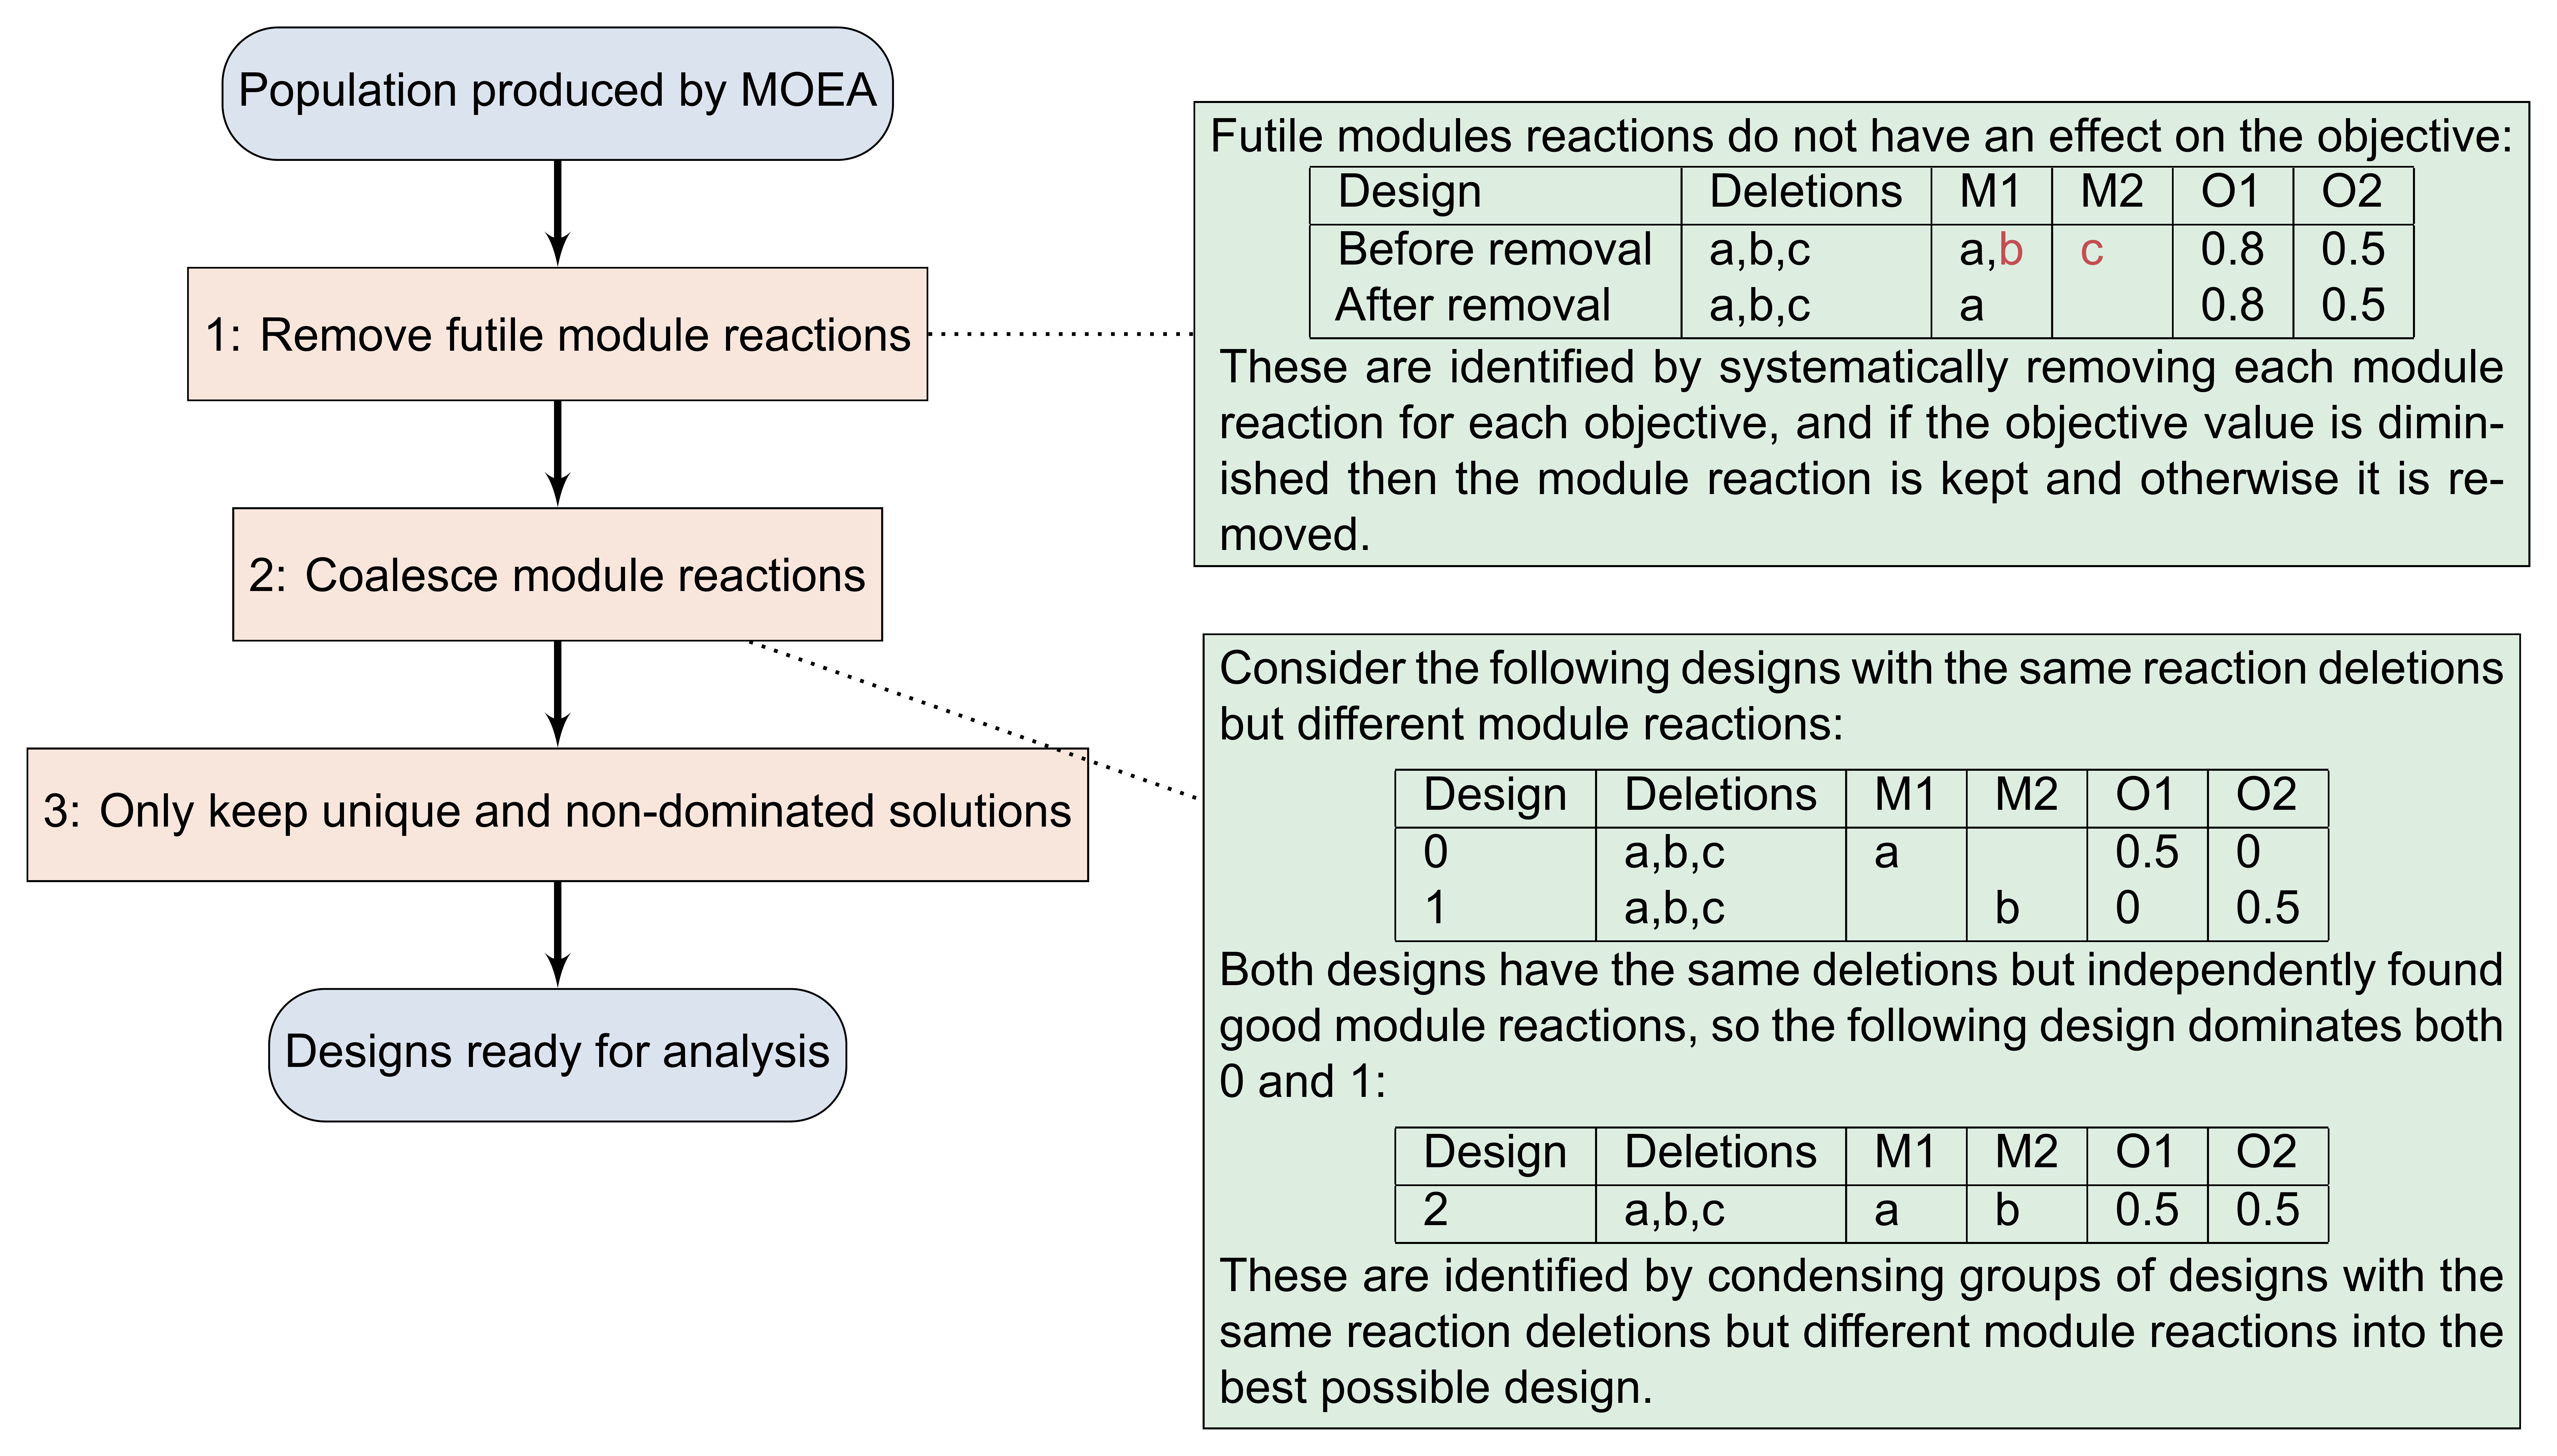
\includegraphics[width=\textwidth,keepaspectratio]{processing.png}
    \caption[Solution improvement process]{Solution improvement process.}
    \label{fig7:processing}
\end{figure}

\begin{figure}[H]
    \centering
    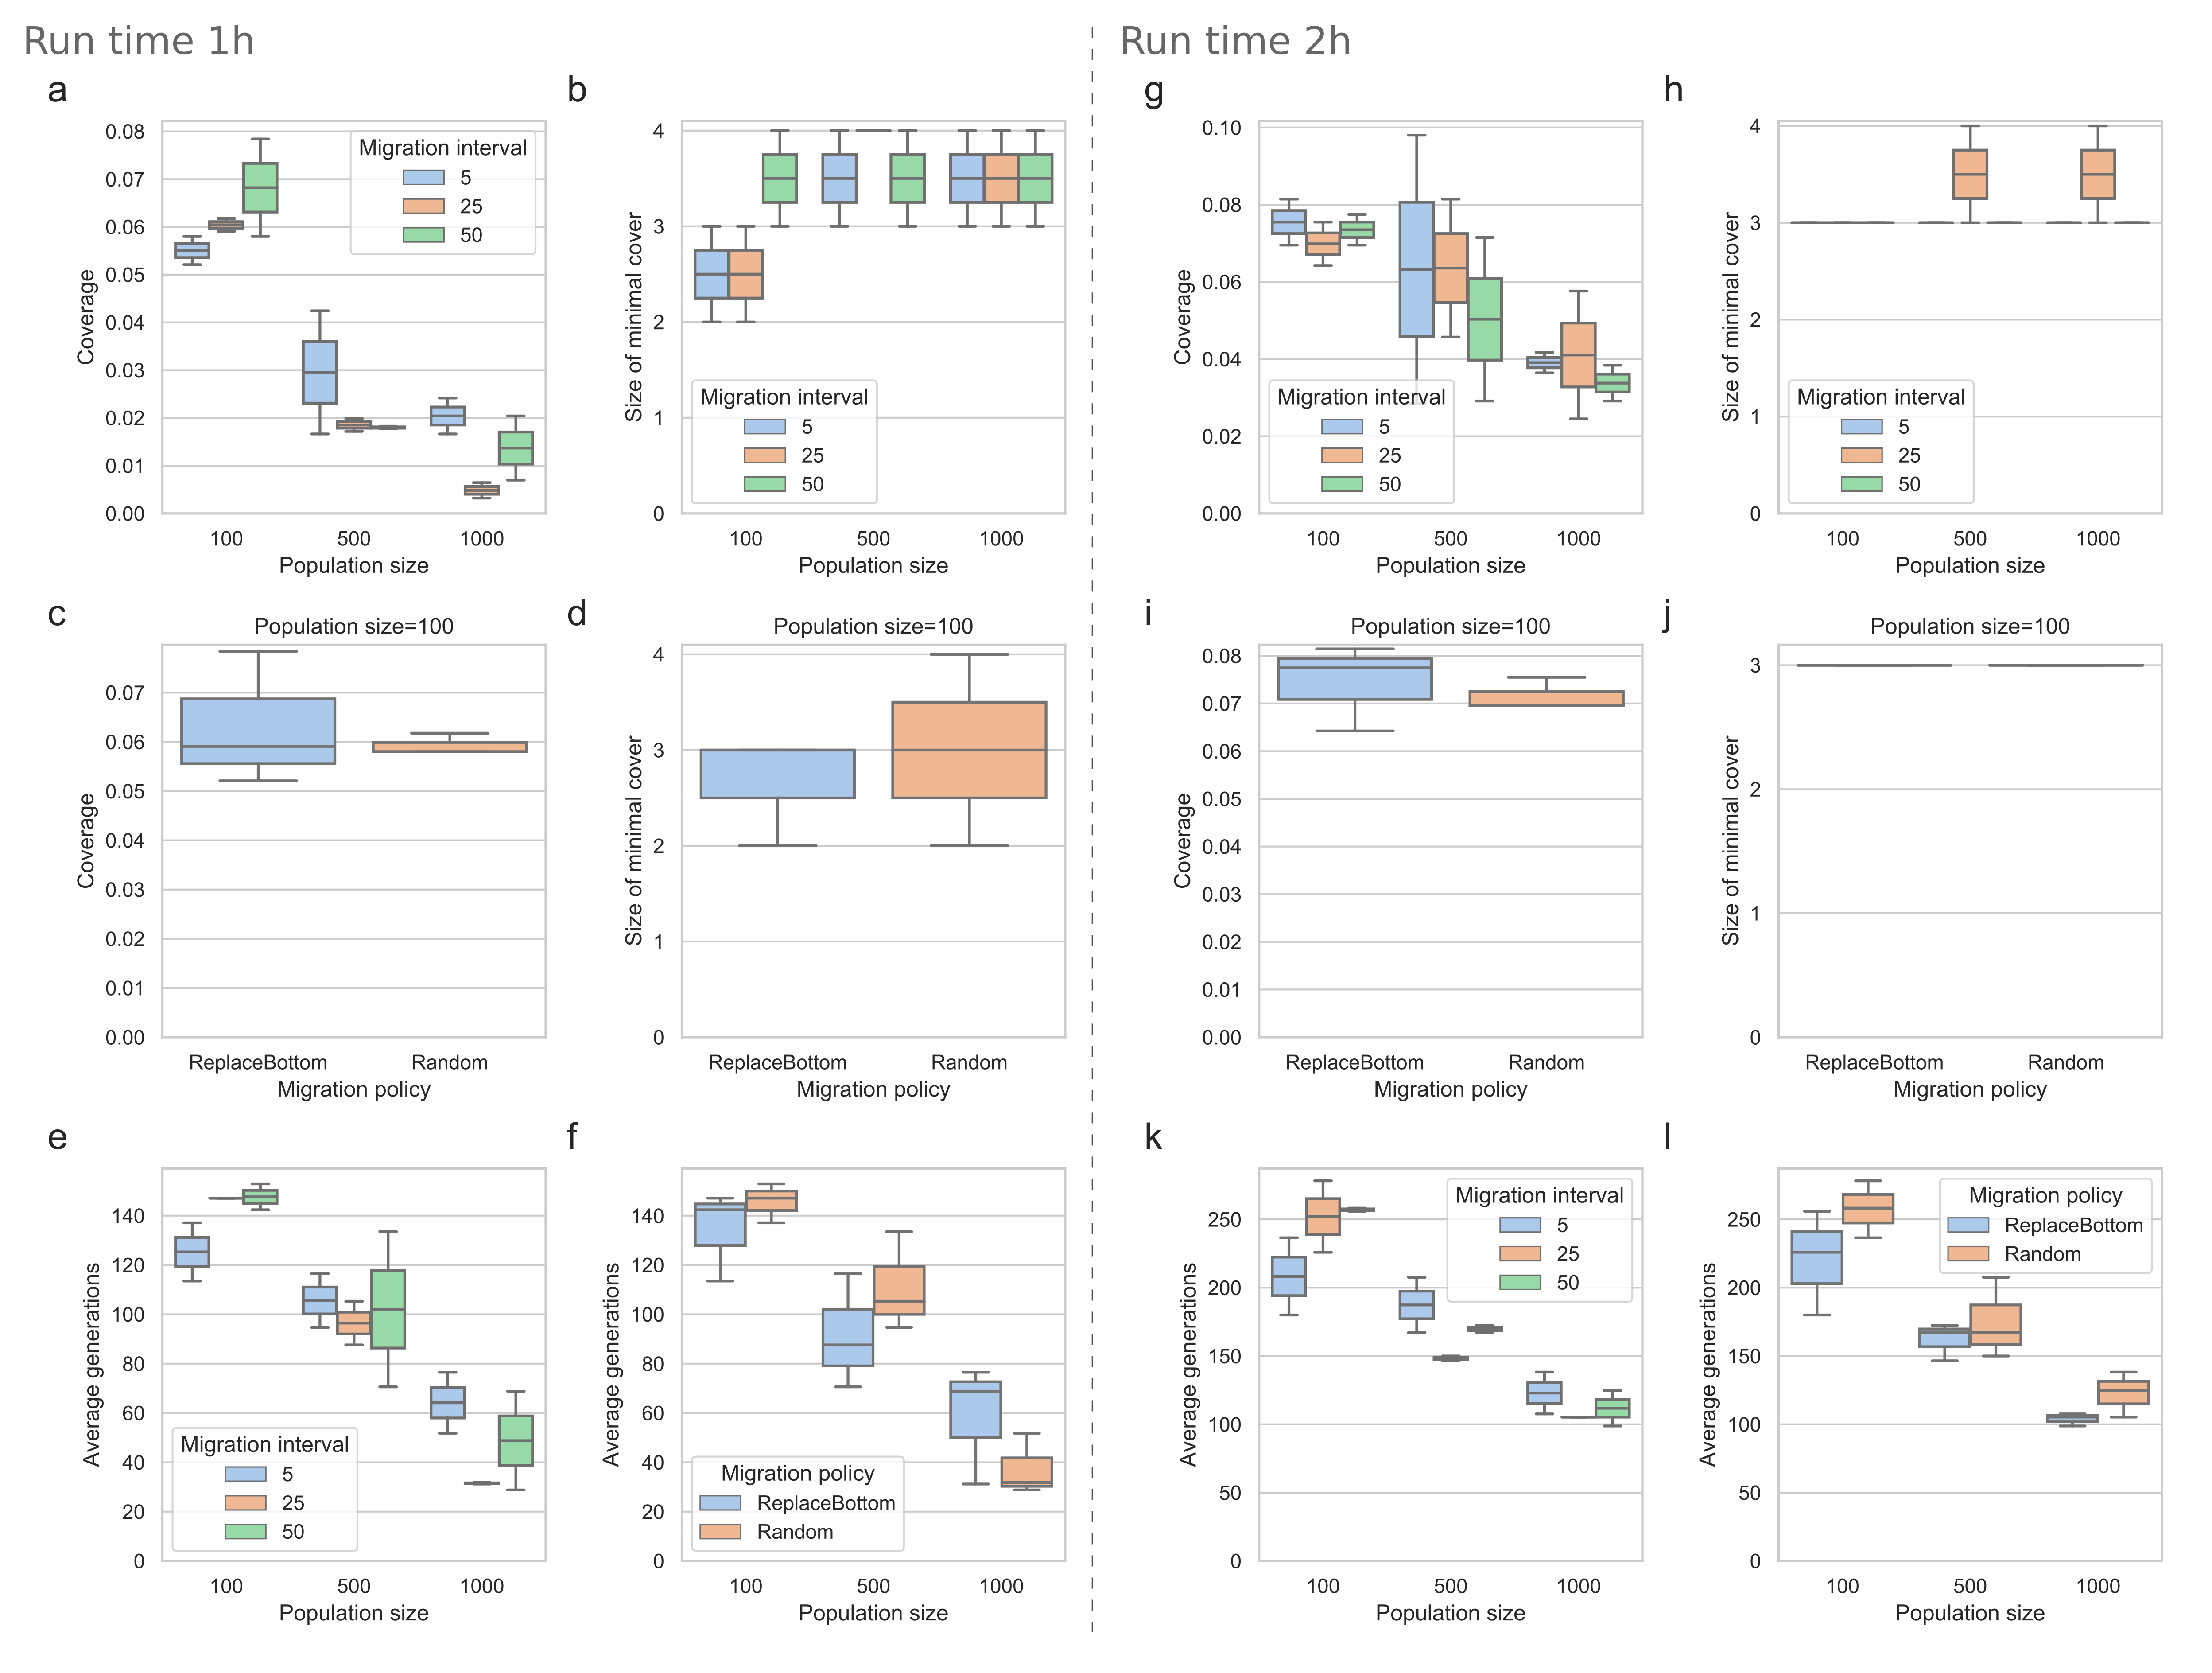
\includegraphics[width=\textwidth,keepaspectratio]{benchmark-gem-model.png}
    \caption[Island-MOEA benchmarking with 20 products]{Island-MOEA benchmarking with 20 products and design parameters $\alpha=6, \beta=1$. For a given run time, this analysis scans through all the combinations of migration interval, migration policy, and population size, hence the data is represented through boxplots since there are too many dimensions to isolate unique points. Note that coverage values are not directly comparable between run times since the use a different reference Pareto front.}
    \label{fig7:benchmark-20prod}
\end{figure}

\begin{figure}[H]
    \centering
    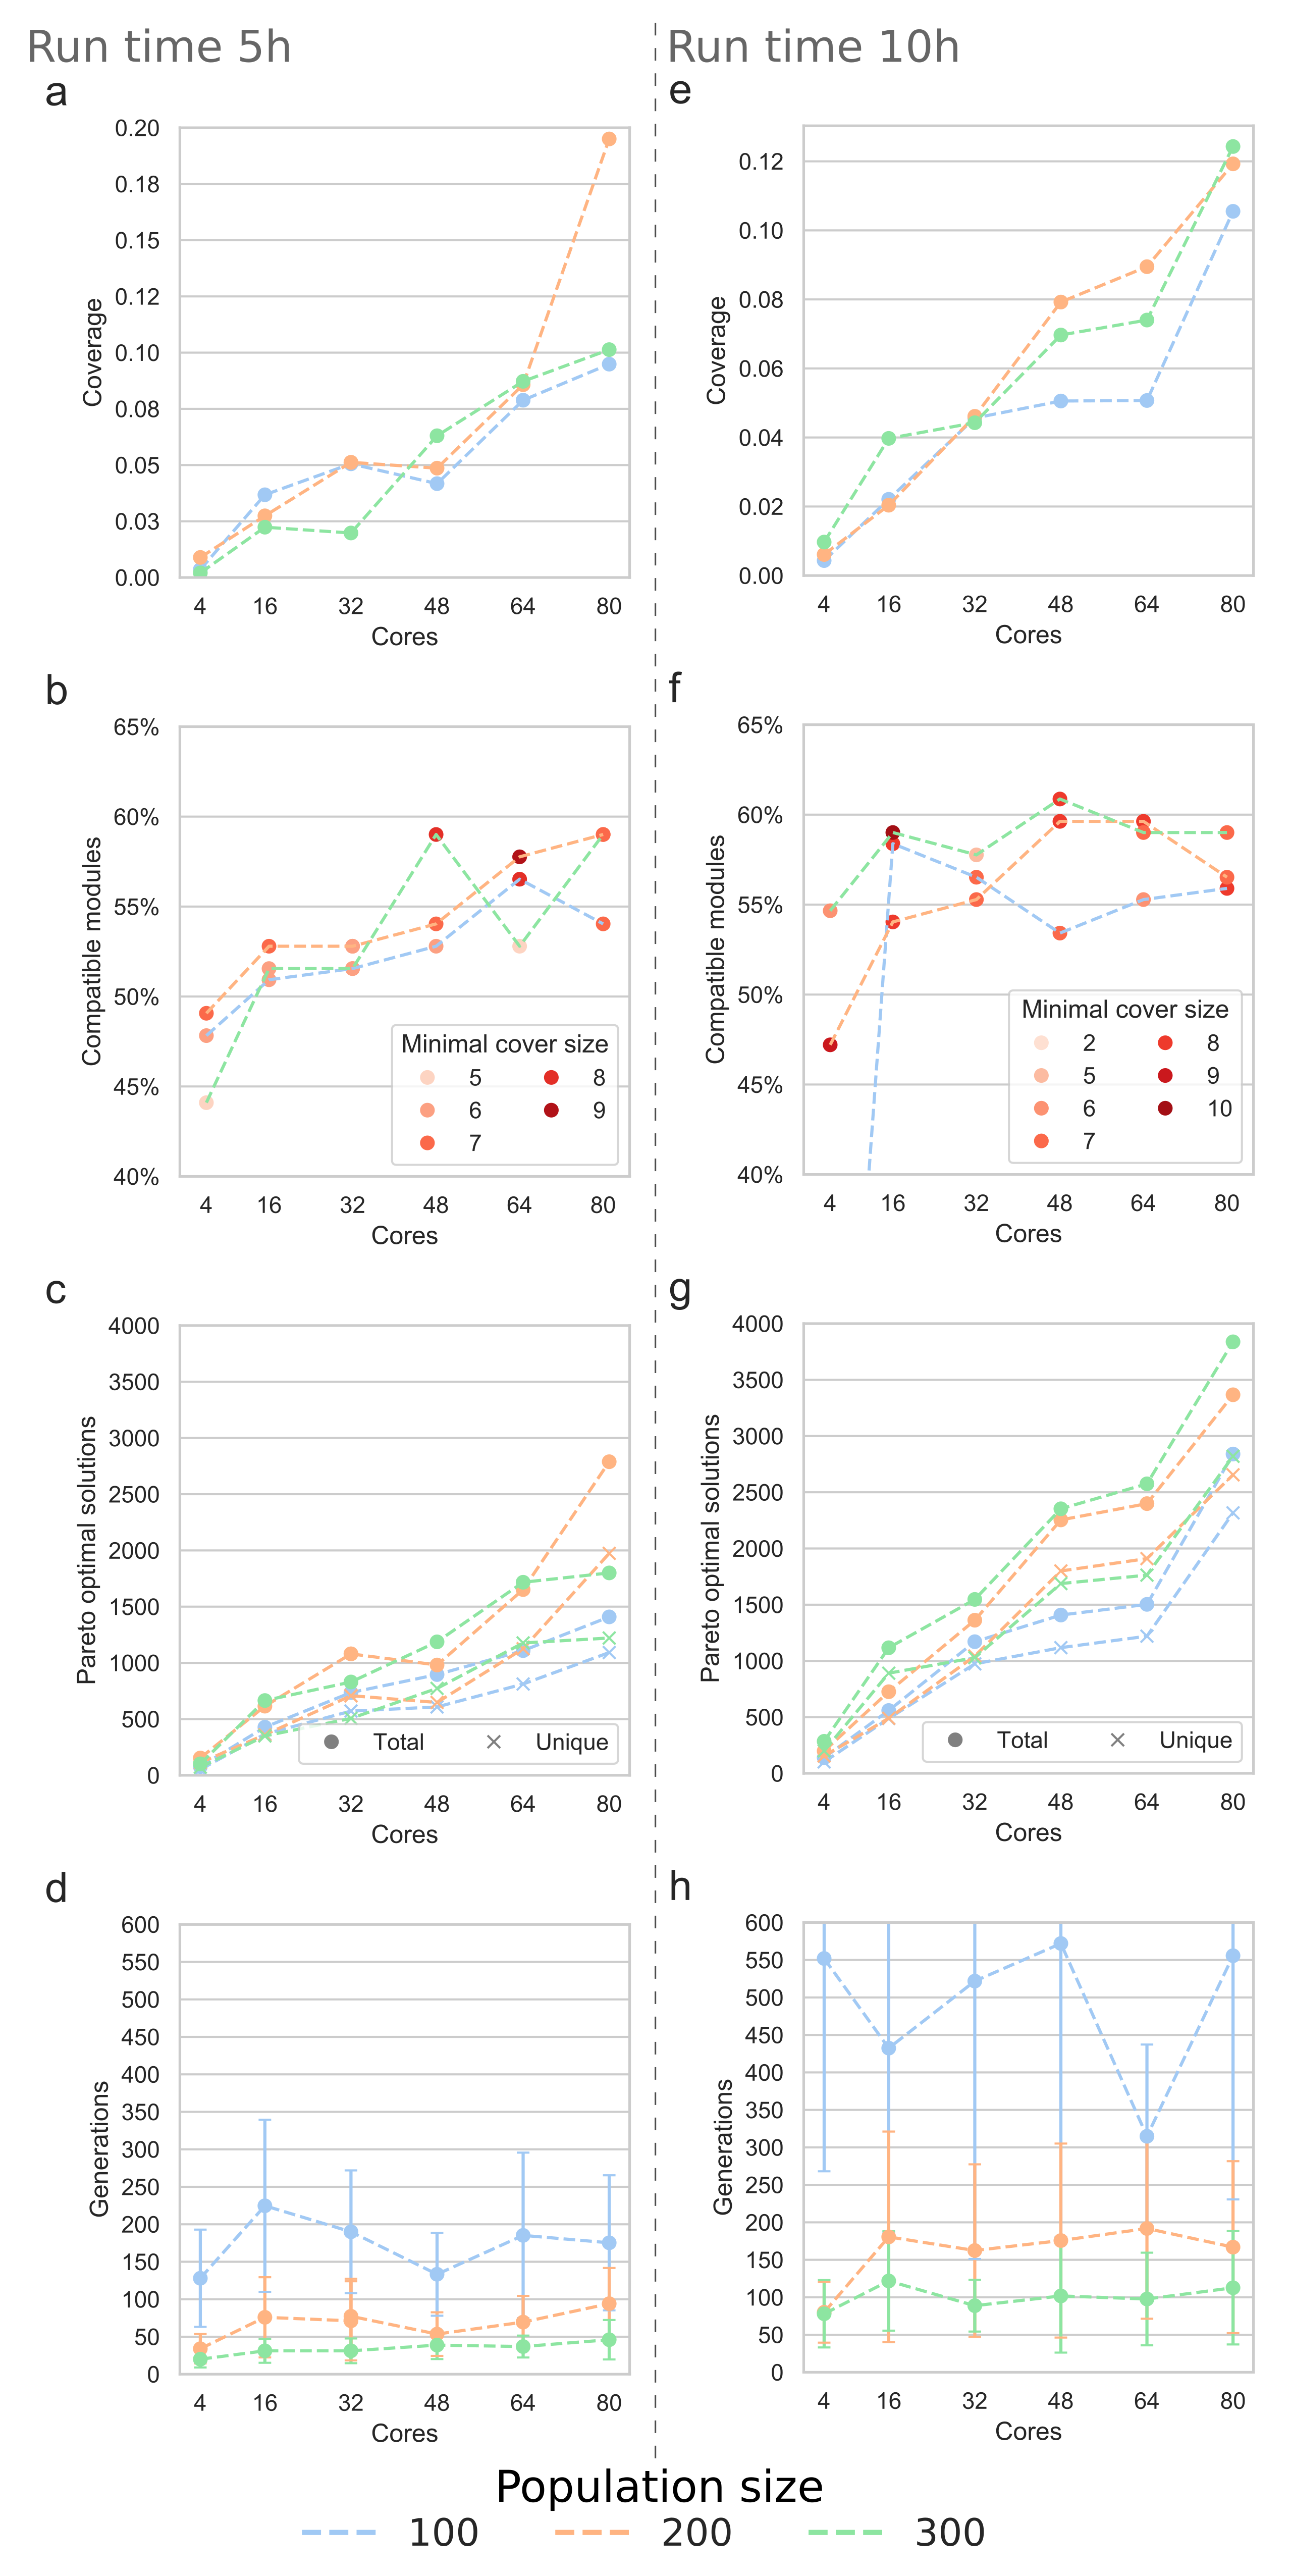
\includegraphics[height=.87\textheight,keepaspectratio]{benchmark-native.png}
    \caption[Island-MOEA benchmarking with 161 products]{Island-MOEA benchmarking with 161 products and design parameters $\alpha=10, \beta=2$. Note that coverage values are not directly comparable between run times since the use a different reference Pareto front. The number of compatible modules indicates the products that appear in at least one design with a design objective above the compatibility threshold, while minimal covers are the smallest number of chassis to ensure all (potentially compatible) products are compatible in at least one of them (Section~\ref{sec:design_characterization}).} %TODO: Explain compatible modules (may also want to describe this in the performance metrics section)
    \label{fig7:benchmark-161prod}
\end{figure}

\begin{figure}[H]
    \centering
    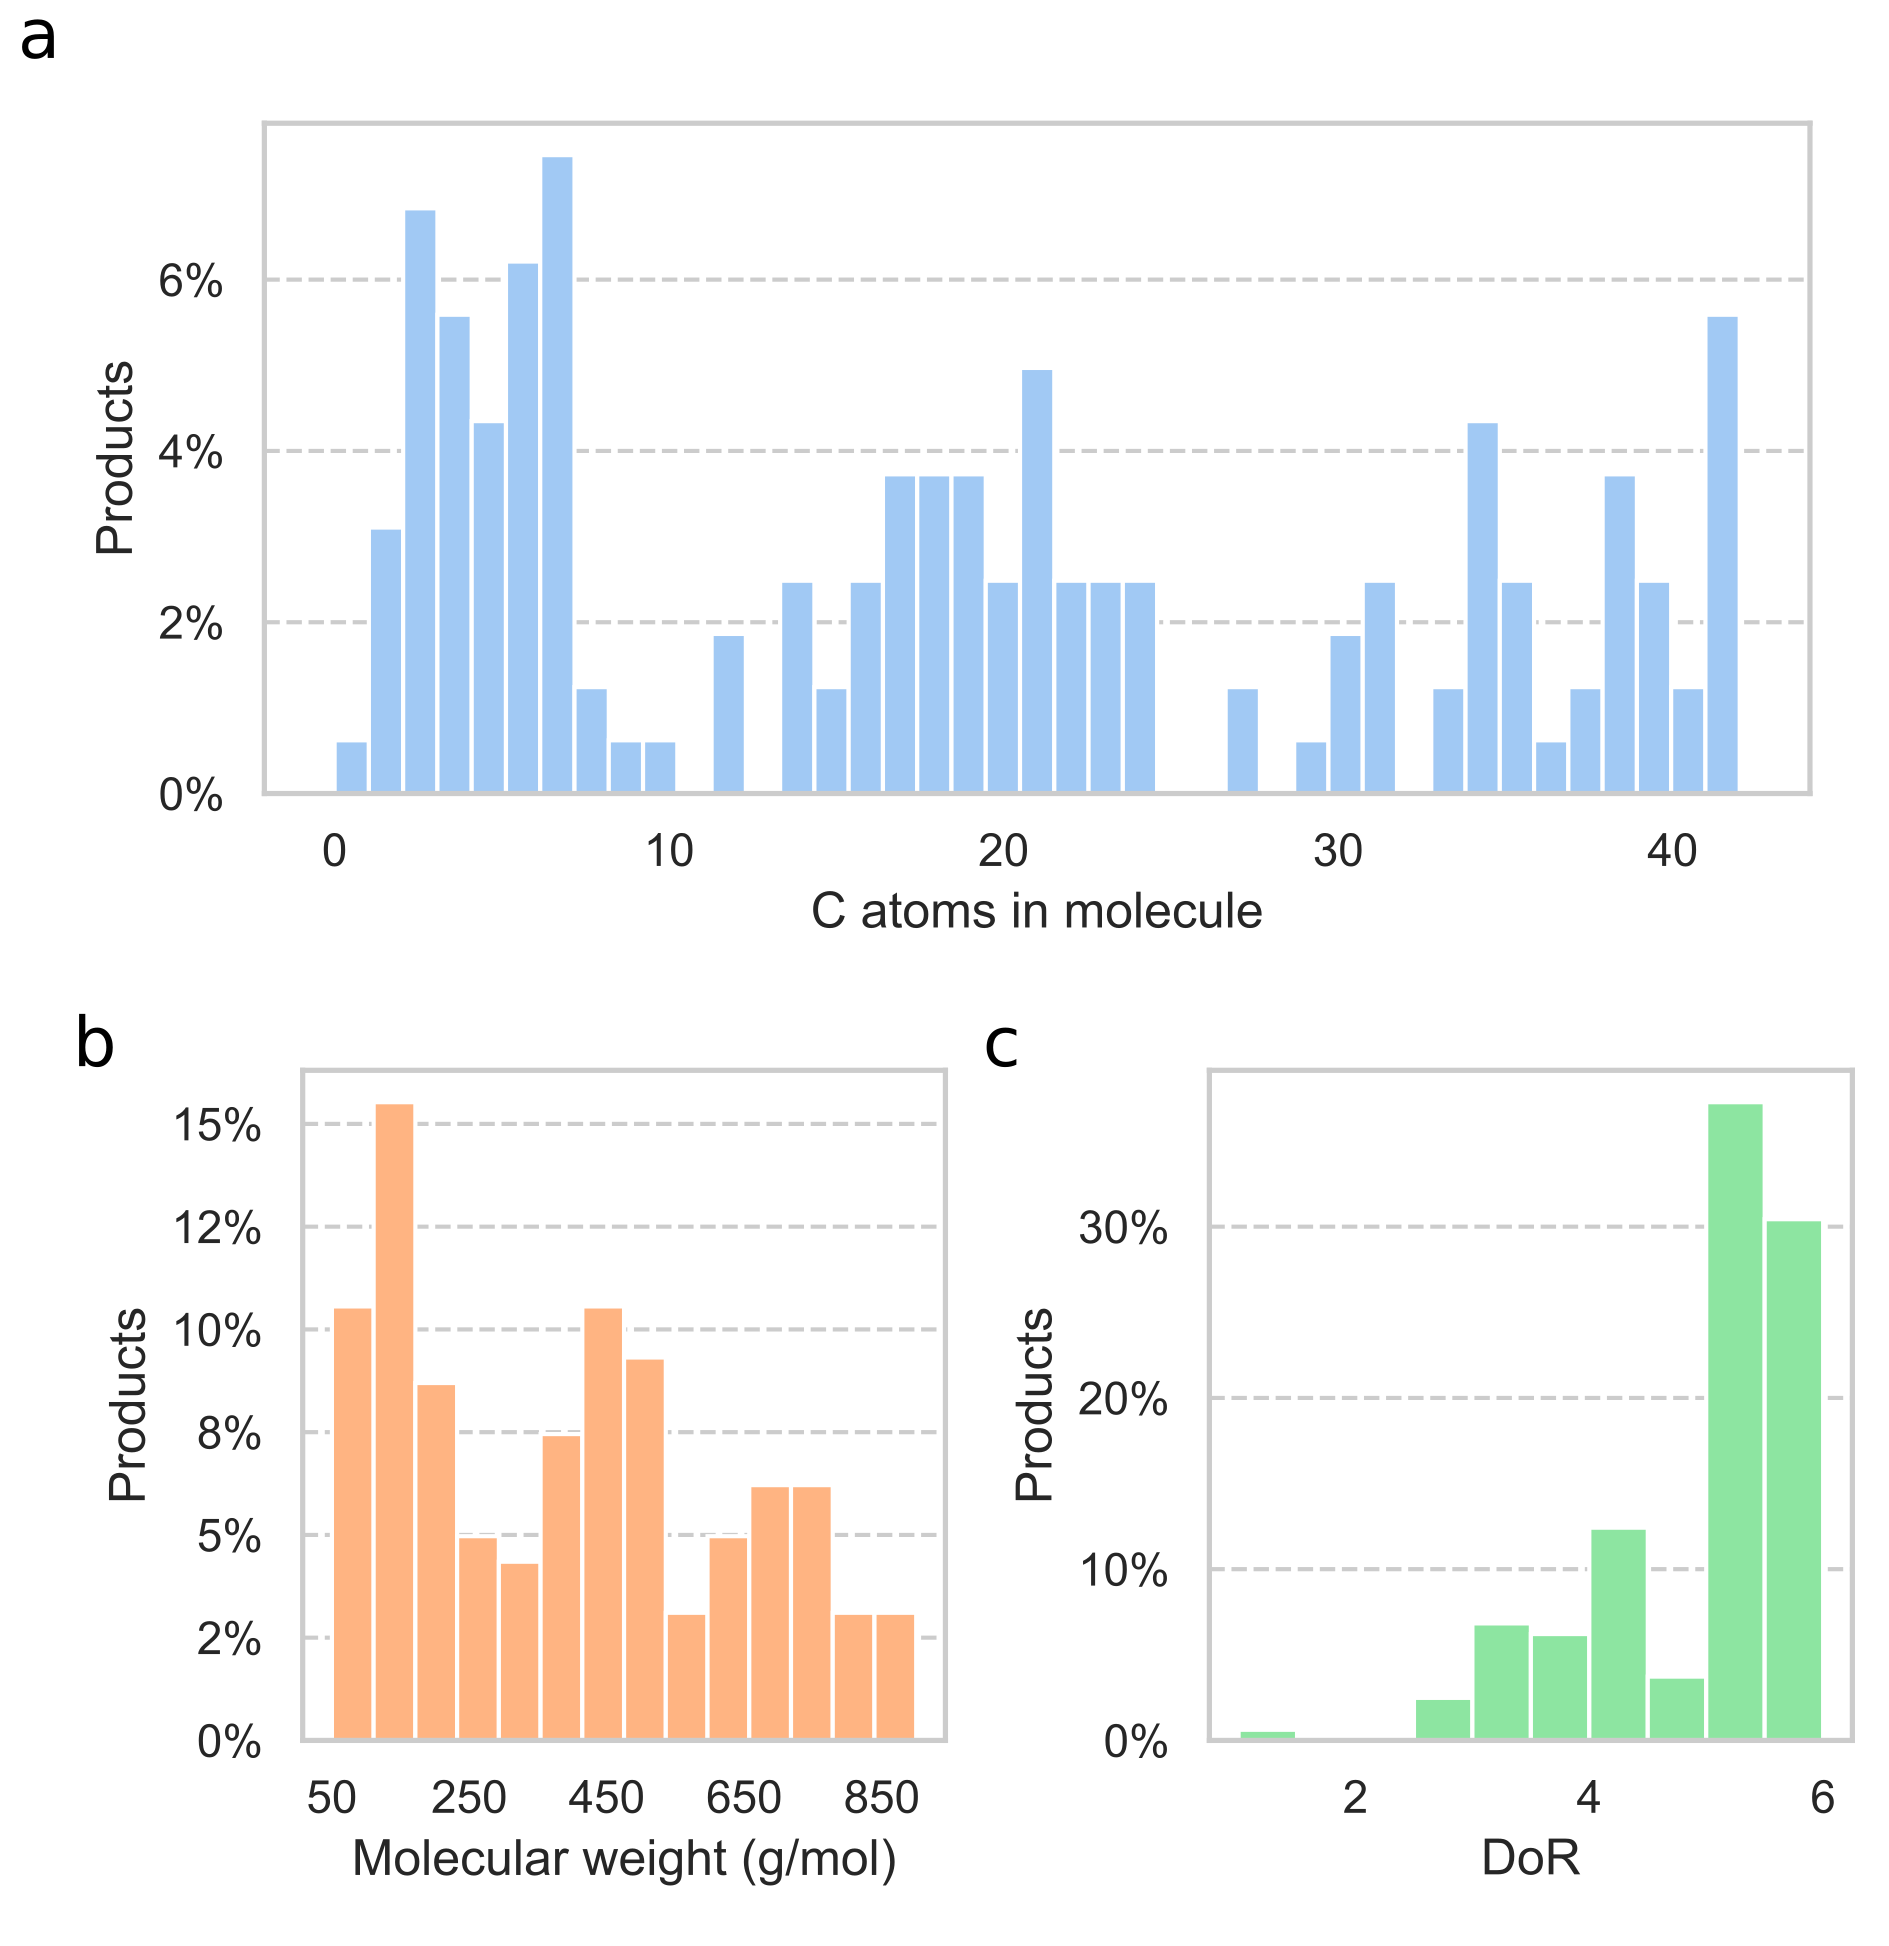
\includegraphics[width=.8\textwidth,keepaspectratio]{biochemical-native.png}
    \caption[Chemical properties of the product library]{Chemical properties of the product library. DoR is the degree of reduction (mol e\textsuperscript{-}/ mol C), which is computed assuming a constant valency of 4,1,-2, and 5 for C,H,O, and P, respectively.  For reference, ethanol has 2 carbon atoms, a molecular weight of 46 g/mol, and a DoR of 6 (mol e\textsuperscript{-}/mol C). The molecular weight and the number of carbon atoms have a Pearson correlation coefficient (pcc) of 0.98, while DoR and the molecular weight only have a pcc of 0.42.}
    \label{fig7:biochemical-properties}
\end{figure}

\begin{figure}[H]
    \centering
    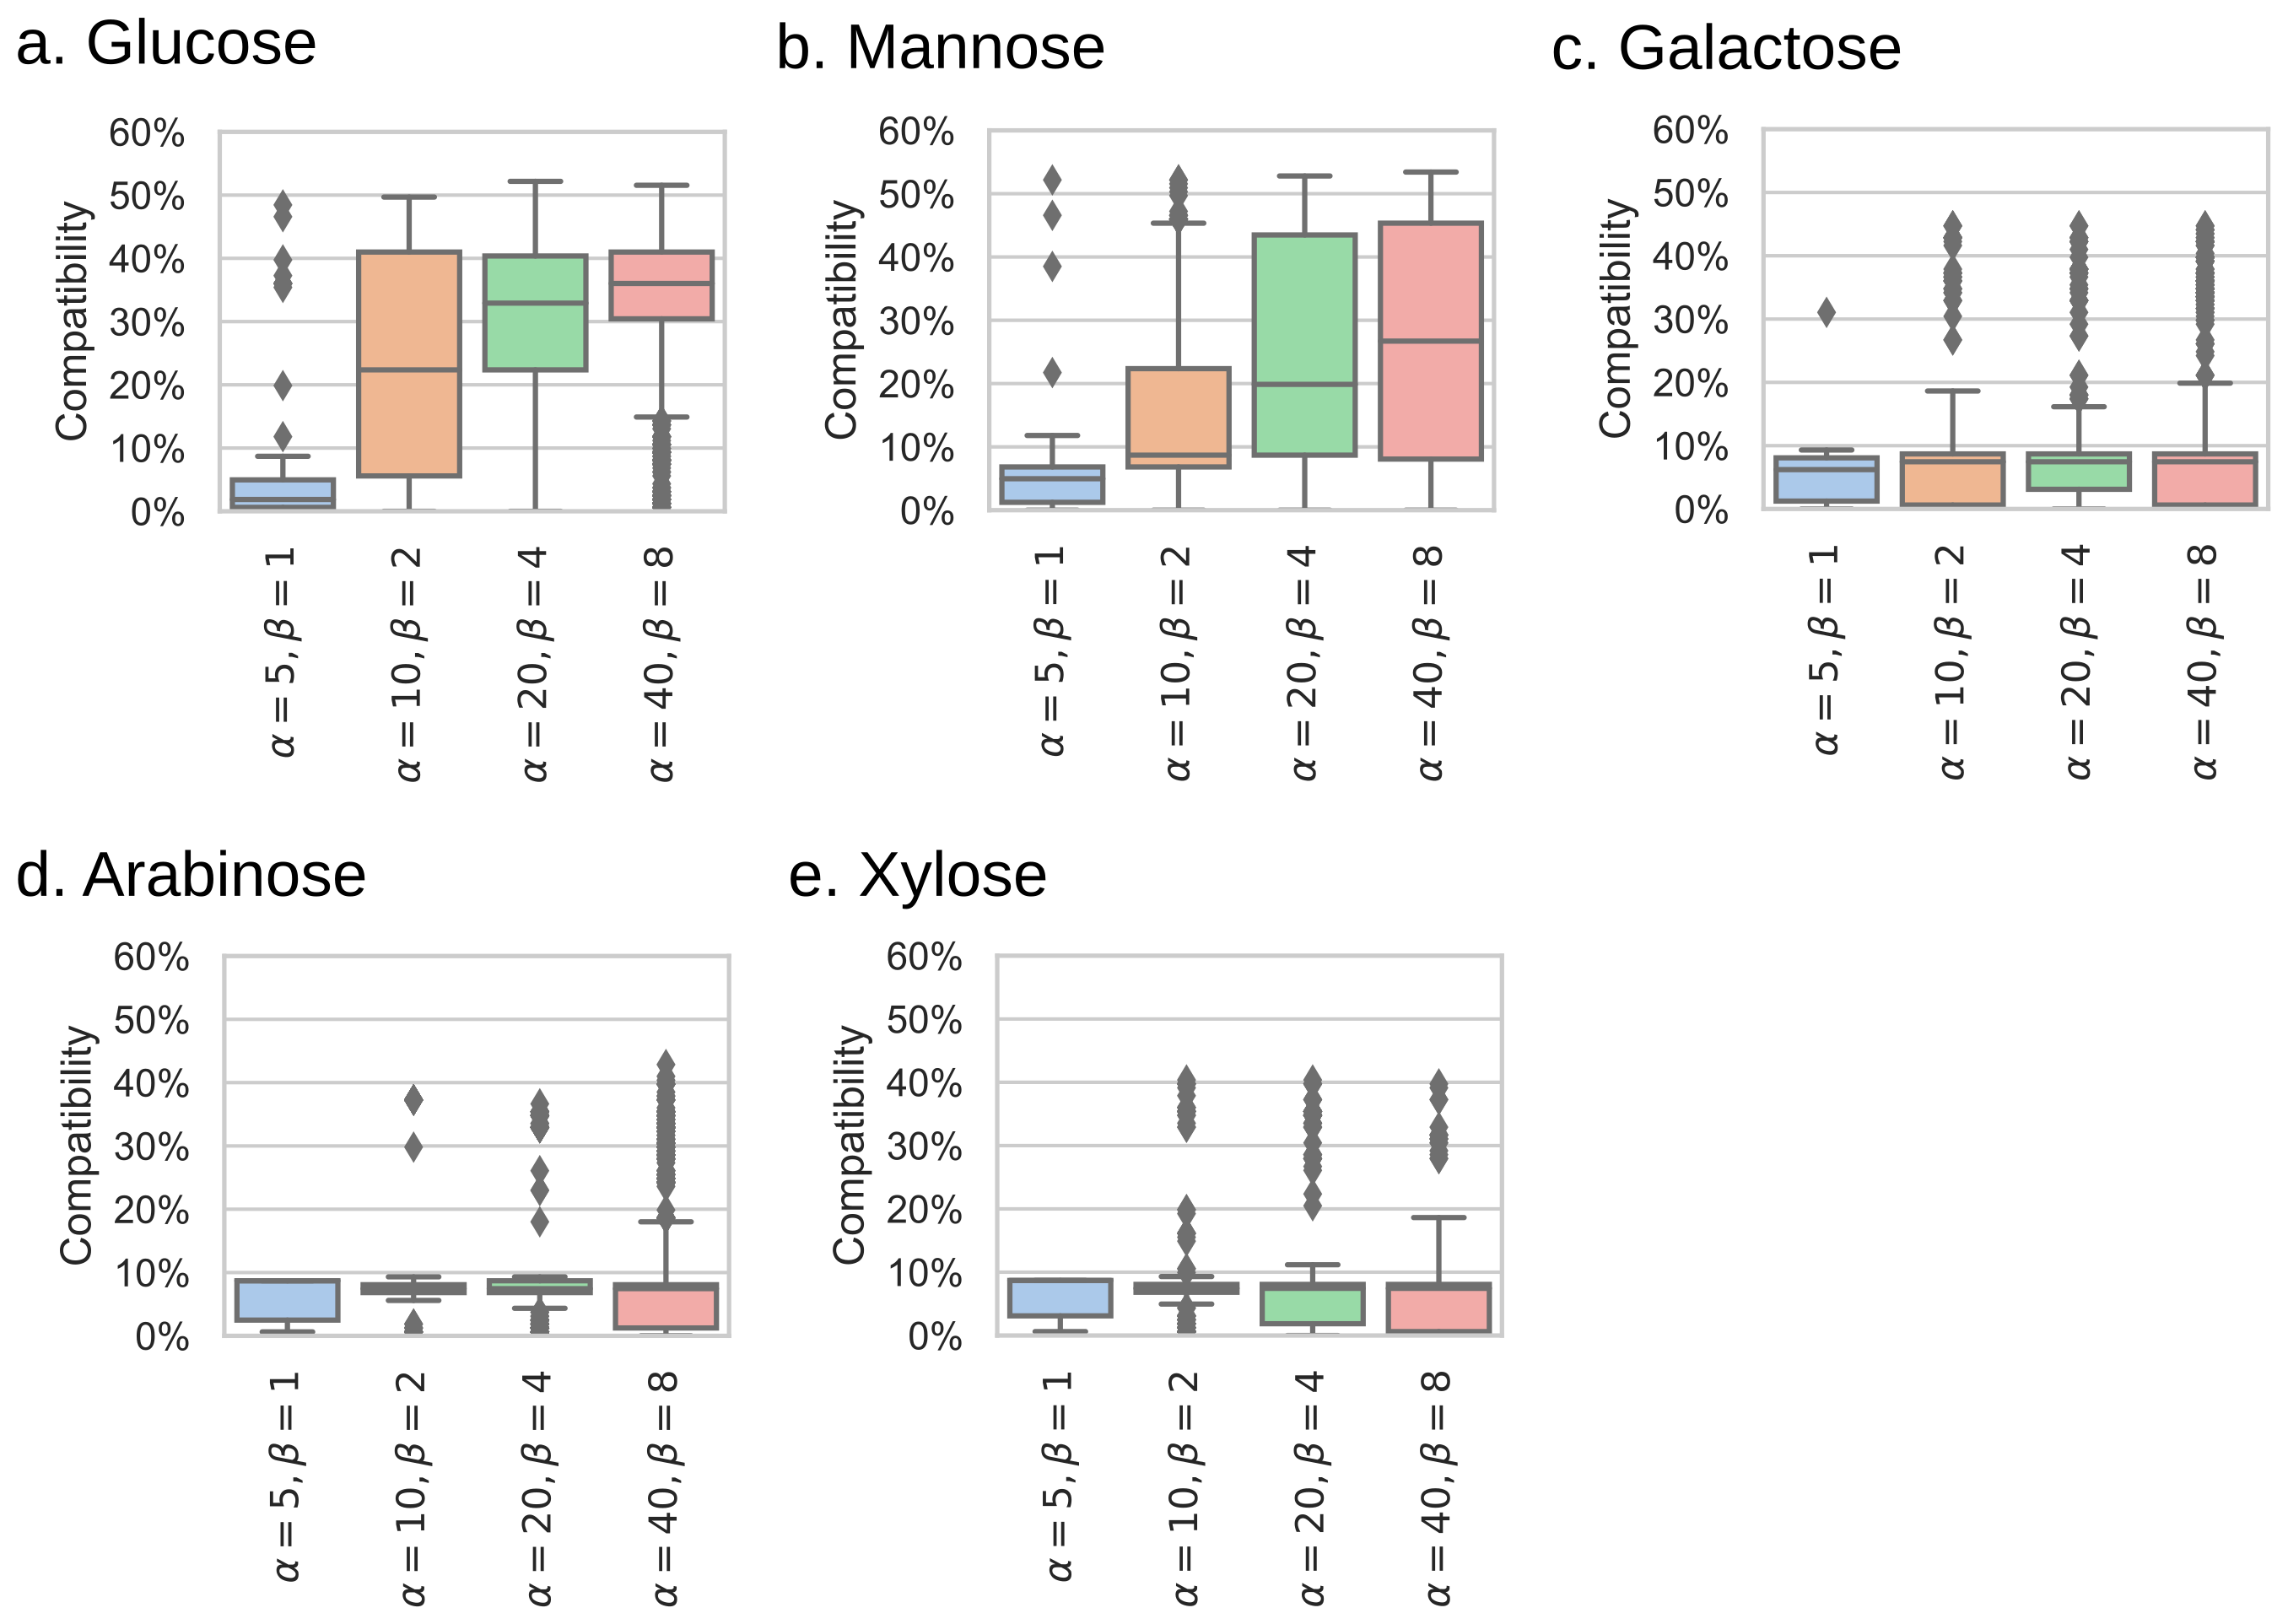
\includegraphics[width=\textwidth,keepaspectratio]{sugars-compatibility.png}
    \caption[Effect of parameters in compatibility distribution]{Compatibility of all designs in a Pareto front as a result of the design parameters. Each panel corresponds to a unique carbon source as the only difference in model configuration.}
    \label{fig7:parameter-scan}
\end{figure}


\begin{figure}[H]
    \centering
    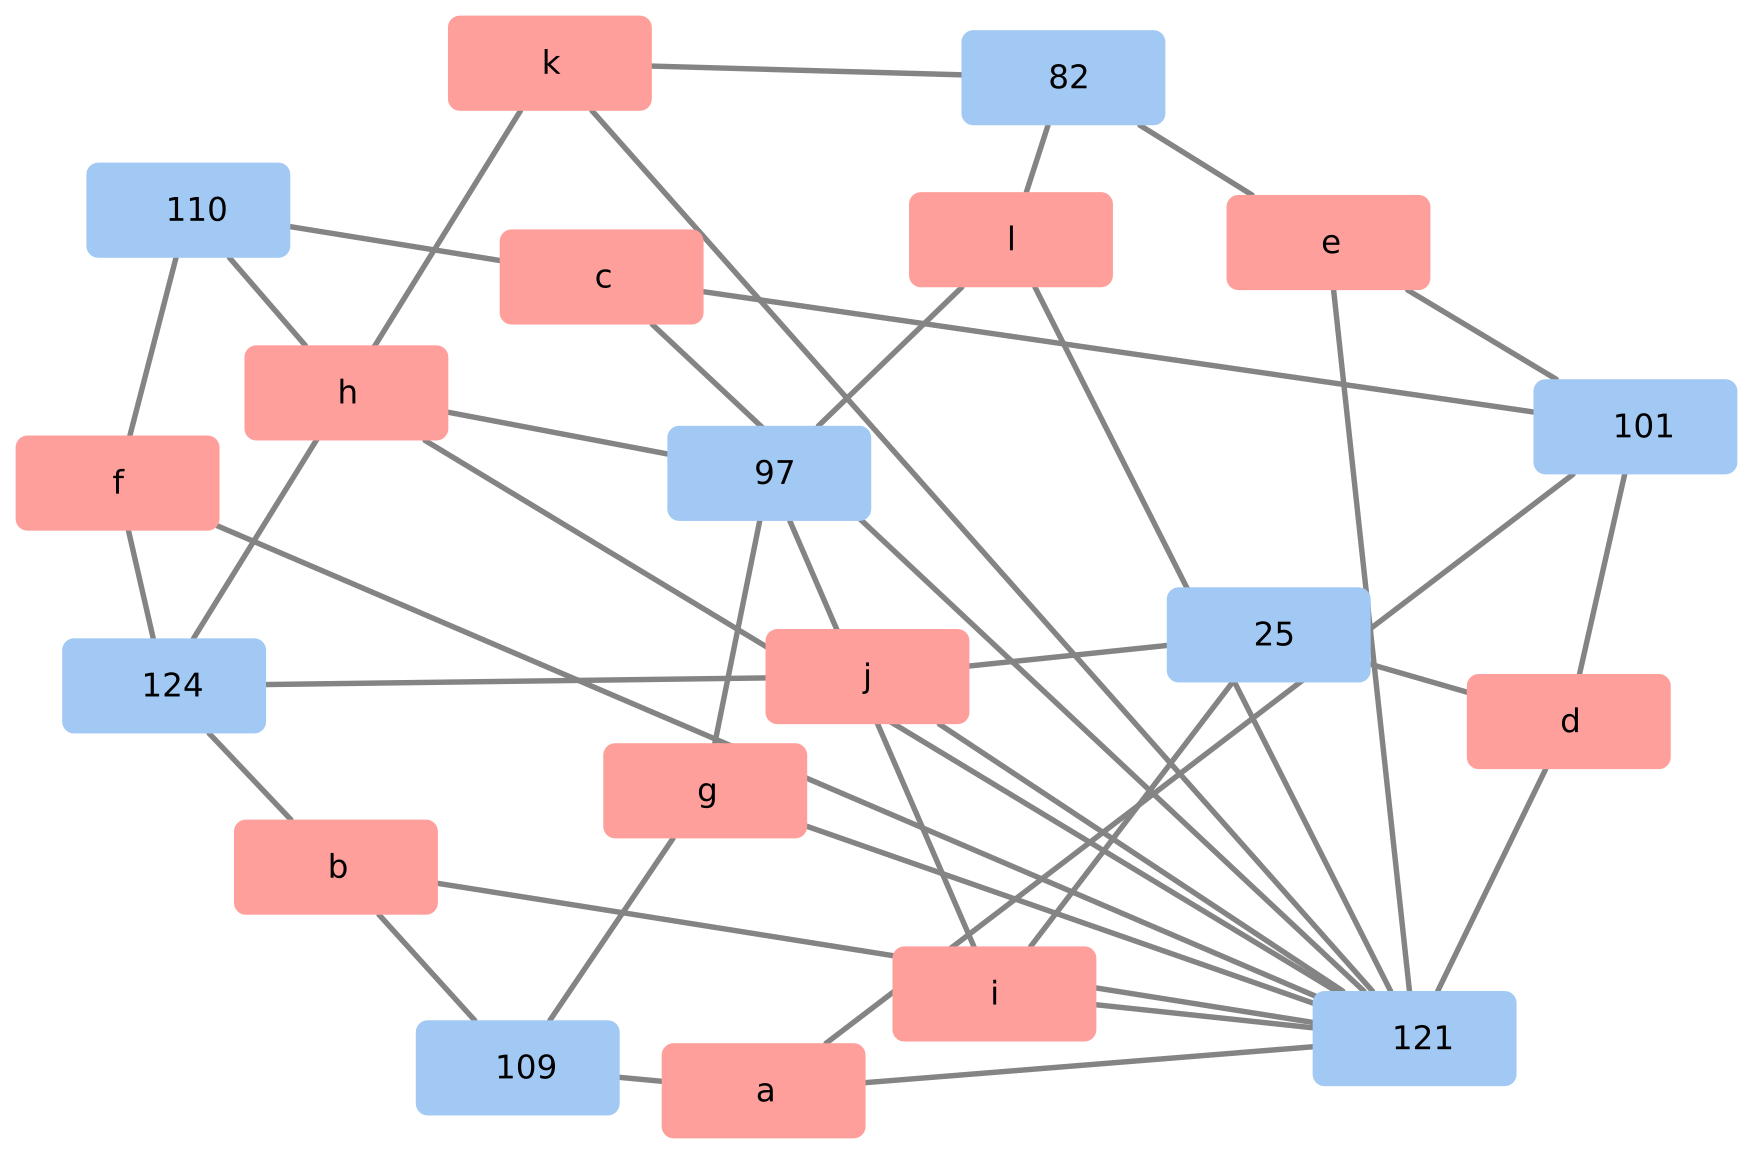
\includegraphics[width=\textwidth,keepaspectratio]{cover-graph.png}
    \caption[Bipartite graph representing minimal covers]{Bipartite graph representing minimal covers for design parameters $\alpha=5$ and $\beta=1$. Covers are colored in red and labeled with letters, while designs are colored in blue.
        %Some designs appear in more covers (e.g., 121).
        All minimal covers are:
            a: [101, 109, 121],
            b: [109, 121, 124],
            c: [101, 110, 121],
            d: [25, 101, 121],
            e: [82, 101, 121],
            f: [110, 121, 124],
            g: [97, 109, 121],
            h: [97, 110, 121],
            i: [25, 97, 121],
            j: [25, 121, 124],
            k: [82, 121, 124],
            l: [82, 97, 121].
            }
    \label{fig7:cover-graph}
\end{figure}
